% =====================================================================
\section{Method}\label{sec:method}
% =====================================================================
This section describes the NITSCI model (Fig.~\ref{fig:arch}), its training objective, the two-stage training
procedure and the decision rule. Given an image $x\in\mathbb{R}^{3\times448\times448}$, a backbone produces
a feature map that is turned into $N$ tokens. Two experts process the tokens, exchange information, and are pooled
and fused by a gate; two heads produce a class distribution and a continuous grade.

\begin{figure}[!htbp]
\centering
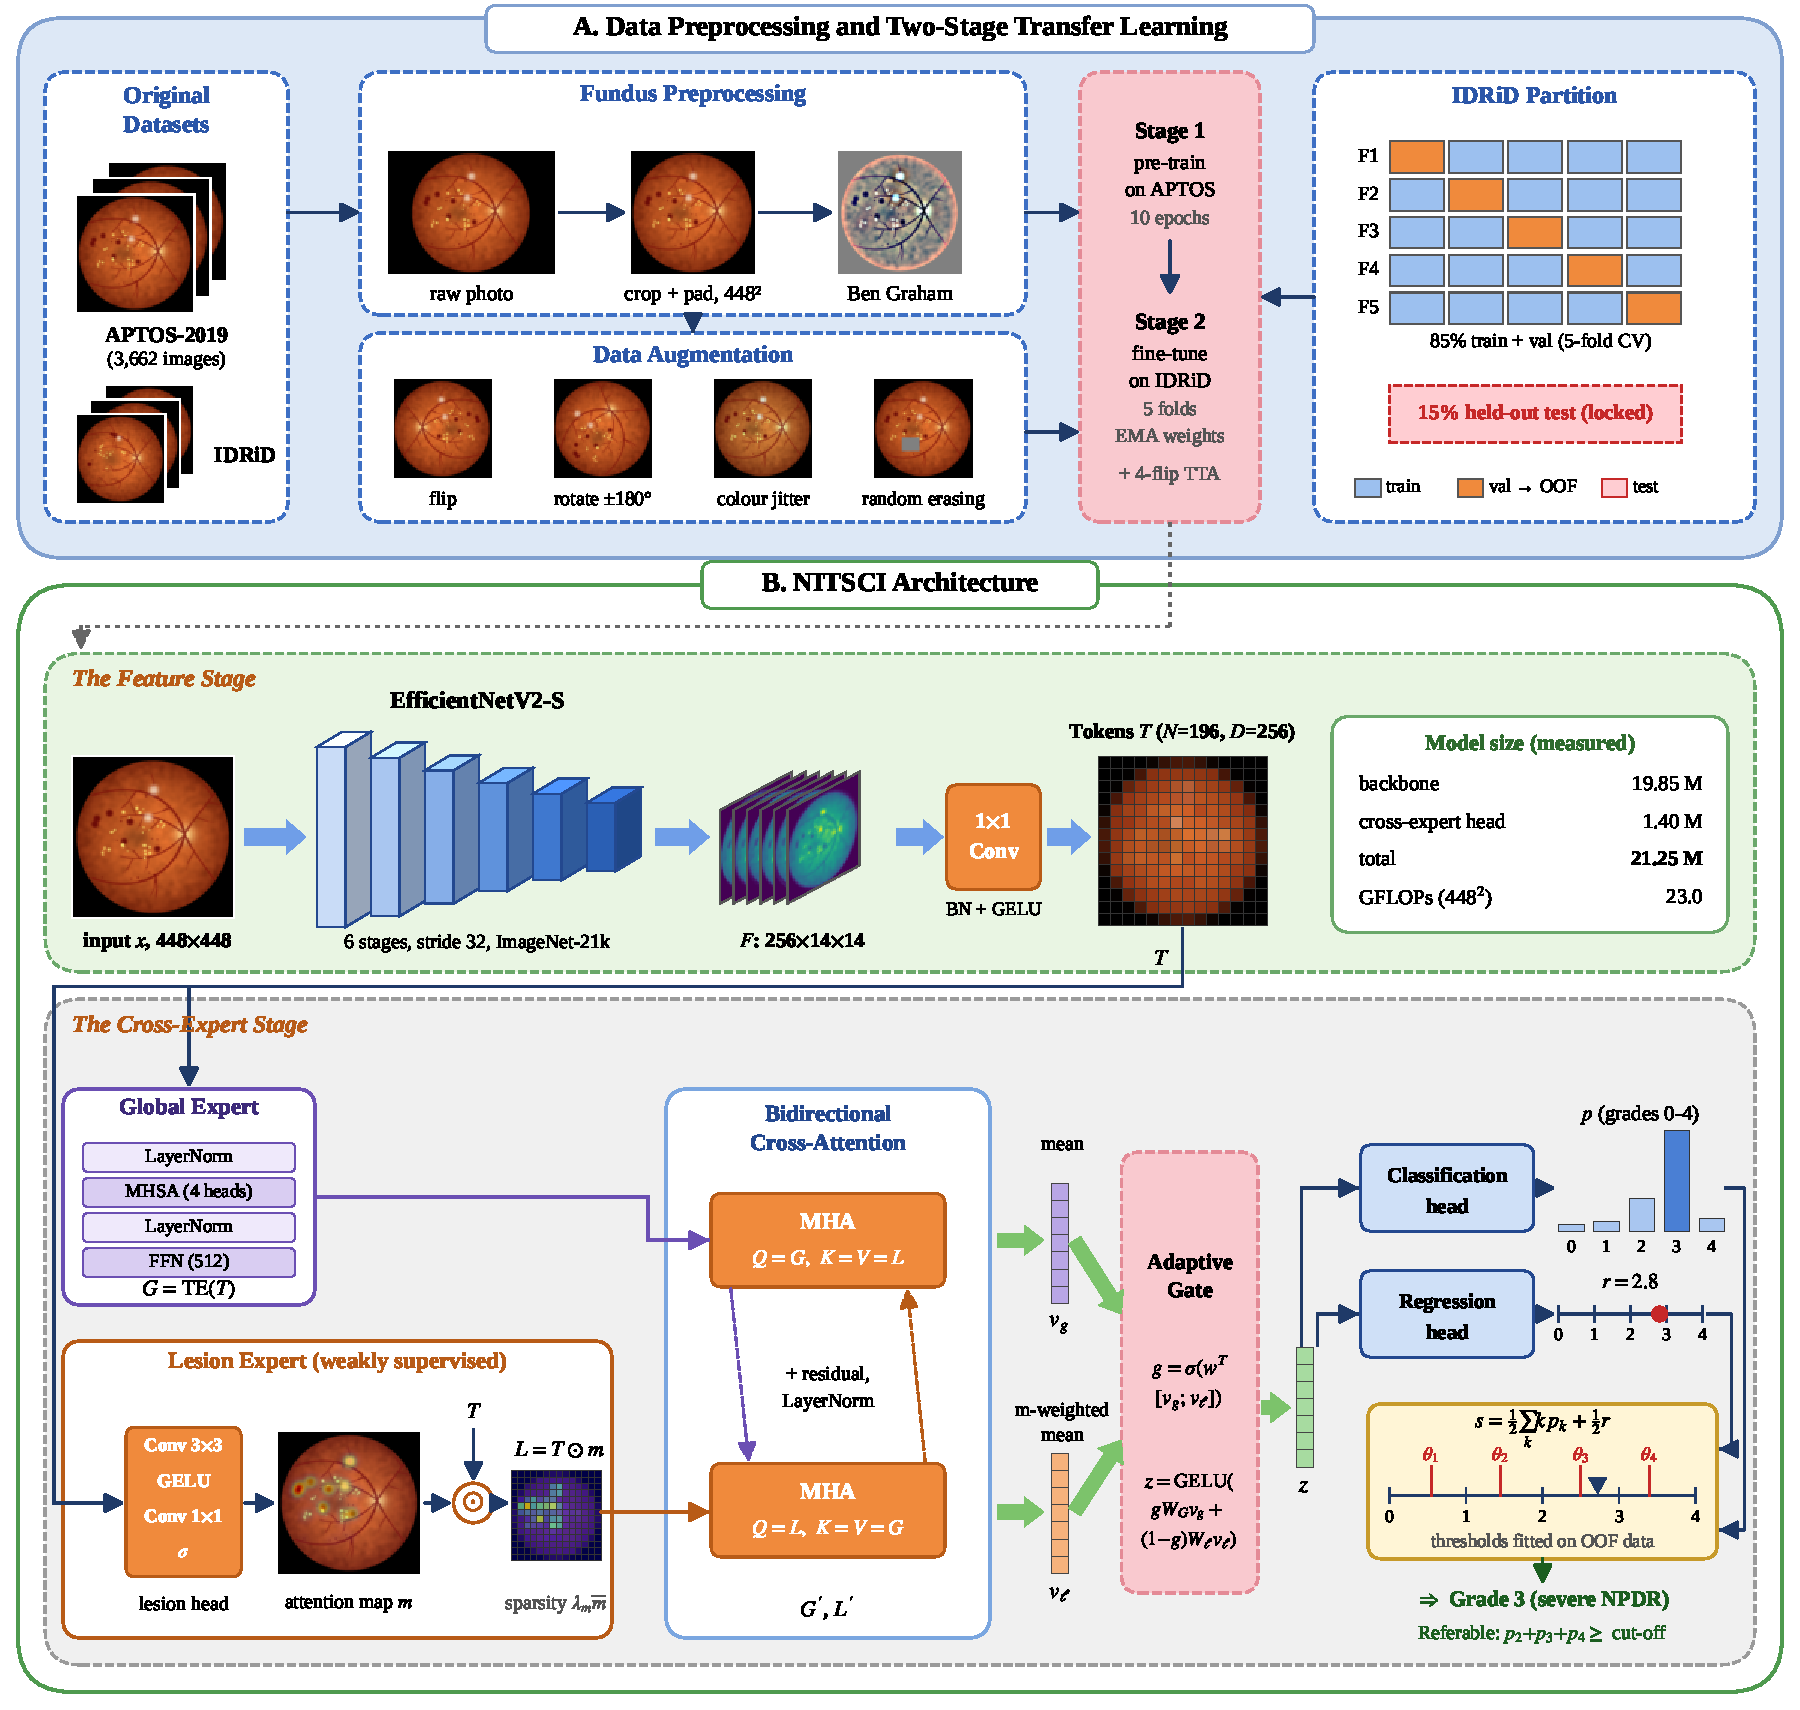
\includegraphics[width=\linewidth]{figures/nitsci_method.pdf}
\caption{Overview of the proposed method. \textbf{(A)} Data preparation and two-stage transfer learning: APTOS-2019
and IDRiD images are pre-processed identically; the full model is pretrained on APTOS-2019 (stage 1) and fine-tuned
on five stratified IDRiD folds (stage 2), while a stratified 15\% IDRiD test set is locked away; out-of-fold
predictions fix the decision rule, the grade thresholds $\theta_1,\dots,\theta_4$ and the referral cut-off.
\textbf{(B)} NITSCI architecture: EfficientNetV2-S features are projected to $N=196$ tokens, processed by a global
expert and by a lesion expert $L=T\odot m$ built from a learned lesion map $m$, coupled by bidirectional
cross-attention, pooled and fused by an adaptive gate $g$; classification and regression heads are combined into the
grade score $s$, whose thresholds come from panel A. Fundus photographs, feature maps and the probability
values shown are synthetic illustrations, not patient data or model outputs.}
\label{fig:arch}
\end{figure}

\subsection{Backbone and tokenisation}
We use EfficientNetV2-S \citep{tan2021efficientnetv2} pretrained on ImageNet-21k and fine-tuned on ImageNet-1k
\citep{ridnik2021imagenet21k}, taken from the \texttt{timm} library \citep{wightman2019timm}. Its last stage
(stride 32, 256 channels) gives a $14\times14$ map for a $448\times448$ input. A $1\times1$ convolution with batch
normalisation and GELU projects it to $F\in\mathbb{R}^{D\times h\times w}$ with $D=256$, which is flattened into
$N=hw=196$ tokens $T\in\mathbb{R}^{N\times D}$.

\subsection{Lesion-attention map and lesion expert}
A light head ($3\times3$ convolution to $D/4$ channels, GELU, $1\times1$ convolution to one channel, sigmoid)
predicts a spatial map $m\in[0,1]^{h\times w}$. No lesion annotation is used: $m$ is learned end-to-end from grade
labels and is encouraged to be sparse by an $\ell_1$ penalty (Eq.~\ref{eq:loss}). The lesion expert is the
re-weighted token set
\begin{equation}
L = T\odot m, \qquad L_i = m_i\,T_i,\; i=1,\dots,N.
\end{equation}

\subsection{Global expert}
The global expert is one pre-norm Transformer encoder layer \citep{vaswani2017attention} with four heads, a
feed-forward width of $2D$ and dropout 0.1, applied to all tokens: $G = \mathrm{TE}(T)$. It models context across
the whole retina, such as the spatial spread of lesions and their relation to the optic disc and macula.

\subsection{Bidirectional cross-attention}
Each expert queries the other with multi-head attention (four heads, dropout 0.1):
\begin{align}
Z_g &= \mathrm{MHA}(Q{=}G,\;K{=}L,\;V{=}L), & G' &= \mathrm{LN}(G + Z_g),\\
Z_\ell &= \mathrm{MHA}(Q{=}L,\;K{=}G,\;V{=}G), & L' &= \mathrm{LN}(L + Z_\ell).
\end{align}
The global stream thus gathers lesion evidence, and the lesion stream receives the context needed to interpret it.

\subsection{Pooling and adaptive gate}
The global stream is mean-pooled, $v_g = \frac1N\sum_i G'_i$, and the lesion stream is pooled with the lesion
weights, $v_\ell = \sum_i m_i L'_i \big/ (\sum_i m_i + \epsilon)$. A scalar gate decides, per image, how much each
expert contributes:
\begin{equation}
g = \sigma\!\left(w^\top[v_g; v_\ell] + b\right),\qquad
z = \mathrm{GELU}\!\left(g\,W_G v_g + (1-g)\,W_L v_\ell\right).
\label{eq:gate}
\end{equation}
This is a two-expert soft mixture \citep{jacobs1991adaptive}; $g$ is also reported for interpretability.

\subsection{Dual head and grade score}
Two heads share $z$: a classification head (LayerNorm, dropout 0.3, linear) gives logits and probabilities
$p\in\Delta^{4}$, and a regression head of the same form gives $r = f_r(z) + 2$, centred on the middle grade.
Their outputs are combined into a continuous score
\begin{equation}
s = \tfrac12\,\textstyle\sum_{k=0}^{4} k\,p_k + \tfrac12\,r .
\label{eq:score}
\end{equation}
A grade is obtained by comparing $s$ with four ordered thresholds $\theta_1<\dots<\theta_4$:
$\hat y = \#\{j:\ s \geq \theta_j\}$.

\subsection{Training objective}
For a mini-batch the loss is
\begin{equation}
\mathcal{L} = \mathrm{CE}_{w,\varepsilon}(p, y) + \lambda_r\,\mathrm{SmoothL1}(r, y) + \lambda_m\,\overline{m},
\label{eq:loss}
\end{equation}
where $\mathrm{CE}_{w,\varepsilon}$ is cross-entropy with label smoothing $\varepsilon = 0.05$
\citep{szegedy2016rethinking} and class weights $w_c \propto n_c^{-1/2}$ (normalised to mean one, computed on the
training fold), $\overline m$ is the mean of the up-sampled lesion map, $\lambda_r = 0.5$ and $\lambda_m = 0.01$.
The square-root weighting is a compromise between ignoring and fully inverting the imbalance.

\subsection{Two-stage training}
\textbf{Stage 1 (APTOS).} The full model, initialised from ImageNet-21k backbone weights, is trained on APTOS-2019 for
10 epochs (learning rate $3\times10^{-4}$, EMA decay 0.999). \textbf{Stage 2 (IDRiD).} For each of the five folds, a
model initialised from the stage-1 weights is fine-tuned for at most 25 epochs (learning rate $2\times10^{-4}$, EMA
decay 0.99, early stopping with patience 8). In both stages we use AdamW \citep{loshchilov2019decoupled} with weight
decay $10^{-4}$, a backbone learning rate one third of the head learning rate, a one-cycle cosine schedule with 10\%
warm-up \citep{smith2019super}, mixed precision \citep{micikevicius2018mixed}, gradient clipping at norm 2, and an
exponential moving average (EMA) of weights \citep{polyak1992acceleration} that is used for validation and saved.
The checkpoint with the highest sum of validation accuracy and quadratic weighted kappa (fixed thresholds
$0.5,1.5,2.5,3.5$, no TTA) is kept.

\subsection{Inference and decision rule}\label{sec:decision}
Each fold model predicts every test image under four views (identity, horizontal flip, vertical flip, both);
probabilities and regression outputs are averaged over views and over the five folds (20 predictions per image).
The decision rule is chosen \emph{on out-of-fold (OOF) predictions only} among three candidates: (i) argmax of $p$;
(ii) rounding $s$ with thresholds $0.5,1.5,2.5,3.5$; (iii) optimised thresholds, found by coordinate search
(four rounds, 80 candidate values per threshold, constrained to remain ordered) maximising OOF accuracy. The chosen
rule was \emph{\res{rule}}, with thresholds (\res{thr}).

\textbf{Referable DR.} For the screening task we use $P(\text{referable}) = p_2 + p_3 + p_4$ and select its
operating threshold on OOF predictions by maximising Youden's $J$ \citep{youden1950index} (selected value
\res{refthr}).

\subsection{Model size and cost}
Table~\ref{tab:cost} lists the parameter counts and floating-point operations, measured with PyTorch
\citep{paszke2019pytorch} on a single $448\times448$ input. The cross-expert head adds 7\% to the parameters of the
backbone.

\begin{table}[!htbp]
\centering\small
\caption{Model size and cost for one $448\times448$ image (FLOPs counted as $2\times$ multiply--accumulates).}
\label{tab:cost}
\begin{tabular}{@{}lcc@{}}
\toprule
Component & Parameters (M) & Notes\\
\midrule
EfficientNetV2-S feature extractor & 19.85 & 256 output channels\\
Cross-expert head (all modules after the backbone) & 1.40 & $D=256$, 4 heads\\
\textbf{NITSCI total} & \textbf{21.25} & 23.0 GFLOPs\\
Plain baseline (same backbone, GAP, same dual head) & 19.92 & --\\
\midrule
Inference latency per image (fp16, batch 16, \res{gpu}) & \multicolumn{2}{l}{\res{mspi} ms per model and view}\\
\bottomrule
\end{tabular}
\end{table}
\sectionend{method}
